\section{Validation}
\label{sec:validation}

In this section, we use the \bcool specification presented in Listing~\ref{lst:bcoolrunningexample} to coordinate the running example. The application of \bcool operators generates a coordination specification in \ccsl. Listing~\ref{lst:runningexampleccsl} partially shows the generated \ccsl specification. Note that the individual specification are imported (Listing~\ref{lst:runningexampleccsl}: line 3 and 4) whereas the coordination only adds some constraints (Listing~\ref{lst:runningexampleccsl}: line 9). The behavioral model of each model remains untouched. 
	
\begin{lstlisting}[language=moccml,
	caption={Resulting \ccsl specification for the running example},
	label={lst:runningexampleccsl}, 
	basicstyle=\scriptsize\ttfamily, backgroundcolor=\color{LGrey}, numbers=left, xleftmargin=2pt]
ClockConstraintSystem SyncProductTFSM-fUMLOperatorsCoordination {
imports {
	import "coffeeCoin.extendedCCSL" as coffeeCoin;
	import "coffeeAlgorithm.extendedCCSL" as coffeeAlgorithm;
}
	entryBlock mainBlock
	Block mainBlock {
	 Block coffeeCoincoffeeAlgorithmsublock {
		Relation SyncProductselectCoffee_startselectCoffee_occurs [ RendezVous ]
				( ClockA -> "coffeeAlgorithm::selectCoffee_startAction",
				  ClockB -> "coffeeCoin::selectCoffee_occurs")
		Relation SyncProductreleaseCoffee_startActionreleaseCoffee_occurs [ RendezVous ]
				( ClockA -> "coffeeAlgorithm::releaseCoffee_startAction",
				  ClockB -> "coffeeCoin::releaseCoffee_occurs")
					}
				}
			}
\end{lstlisting}    
		
The \ccsl specification can be executed by using TimeSquare~\cite{timesquarebib}. Figure~\ref{fig:coffemachinevcd} illustrates the partial timing output of the execution of the running example. TimeSquare also offers the possibility to obtain by exploration quantitative results on the scheduling state-space (see Figure~\ref{?}). The state space is always computable if models are finite. 
	 
\begin{figure}[h]
	 	\center
	  	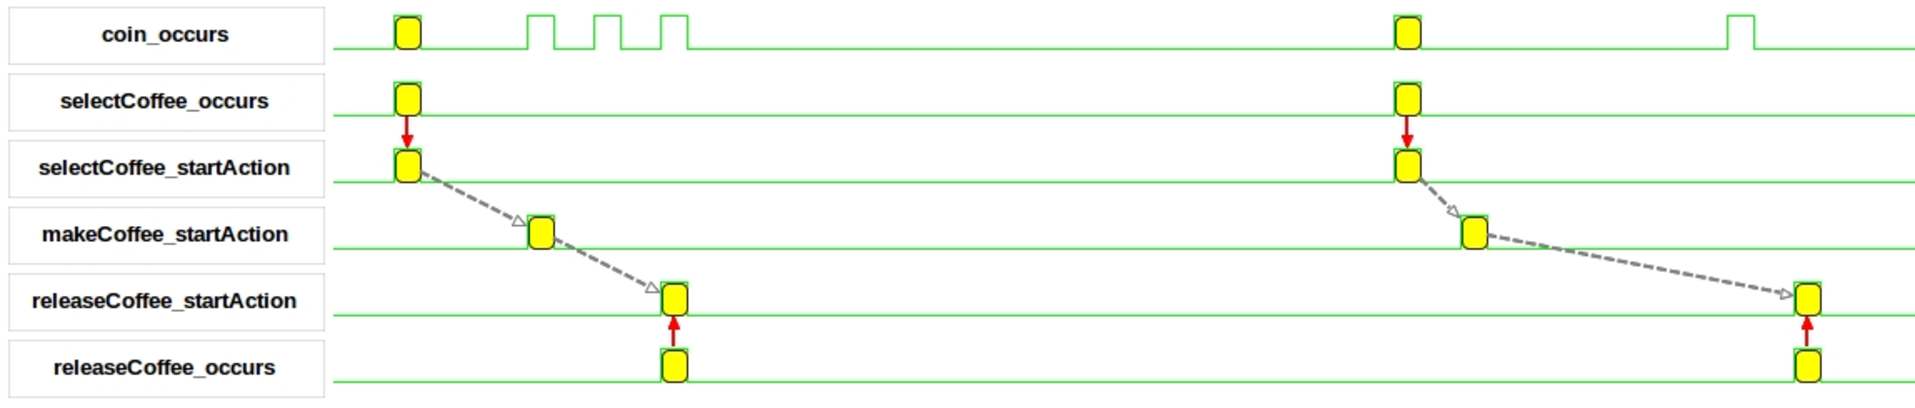
\includegraphics[width=.9\textwidth]{bcool/figs/coffeemachinevcd}
	  	\caption{Resulting timing execution of the coordinated system}
	  	\label{fig:coffemachinevcd}
\end{figure}
	
When a coin is inserted (\emph{coin:occurs} happens), the \emph{selectCoffee:occurs} event is triggered. Then, the coordination forces a simultaneous occurrence between \emph{selectCoffee:occurs} and \emph{selectCoffee:startAction} thus making the activity starts to execute. Then, when the coffee is released, the coordination forces a simultaneous occurrence between the events \emph{releaseCoffee:startAction} and \emph{releaseCoffee:occurs}. The coordination constrains some events by making them to happen simultaneously. This reduces what can be done by individual models, \ie some FSMEvents and Action can only occurs simultaneously. Other events are only constrained by the individual semantics. The coordination constraints the behavior of models without adding new ones. In this sense, the coordination is non intrusive thus not altering the behavior of individual models. 

\todo{To show the space state. To illustrate the last paragraph by showing the state space}

\todo{Recheck state space!}
